
% ---- TITRE ----
\author{Ali Zoubir }
\date{November 2022}

\pagestyle{fancy}

\lhead{ETML-ES}
\chead {\monthyeardate\today}
\rhead{Localisation sous-marine V0.0}


\onecolumn


\begin{figure}
\begin{minipage}{0.47\textwidth}
\centering

\includegraphics[width=.4\textwidth,left,]{../ETML-ES-LOGO.png}
\end{minipage}

\hfill
\begin{minipage}{0.7\textwidth}
\raggedleft
\LARGE \textbf{Localisation sous-marine\\ 2022, V0.0}
\end{minipage}
\end{figure}

\begin{figure}

\hfill


\begin{minipage}{1\textwidth}
% ---- DESCRIPTION ----
\section{Cahier des charges}

\subsection{Description}
L’objectif de ce projet, et de stocker des données de mesures du déplacement d’un module sous-marin par une centrale inertielle, dans le but de mathématiquement le localiser depuis son point de départ (référence). Ceci, car la localisation sous-marine n’est pas une tâche aisée due aux différentes contraintes de communication sous-marine notamment le fait que les ondes électromagnétiques ne s’y propagent pas facilement.
\end{minipage} \vspace{+4mm}

\begin{minipage}{1\textwidth}

\subsection{Aperçu}
    \begin{itemize}
        \item	Sauvegarde d’un set de donnée chaque 100ms.
        \item	Profondeur d’utilisation maximum, de 60m.
        \item	2 heure de logging dans carte SD.
        \item	Sensing sur 9 axes :
        \subitem Mesures [Il est souhaitable que les capteurs choisis aient une faible dérive] ;
        \subsubitem Accéléromètre 3-axes. 
        \subsubitem	Gyroscope 3-axes.
        \subsubitem	Magnétomètre 3-axes. 
        \subsubitem	Senseur de température
        \subsubitem	Profondimètre [0->10bar] [Res 1/10]
        \subsubitem	3 à 5 slots libres MikroE pour autres mesures. 
        \item Possibilité de sauvegarder la localisation de points d’intérêts par :
        \subitem Bouton de sauvegarde [A définir : Magnétique, Optique, Mécanique ou autre].
        \item Batterie, autonomie minimum de 2 heures [$\sim$10$\degree$C].
        \item Charge de la batterie par connecteur USB.
        \item (Optionnel) Lecture des données par connecteur USB (Interfaçage électronique, software optionnel dans cette version).
        \item (Optionnel) Interface LED ou petit écran.\\
    \end{itemize}


\end{minipage}

\end{figure}


\clearpage





% ---- TACHES ----
\subsection{Tâches à réaliser}
Développement et intégration d’un PCB avec capteurs et logging sur carte SD dans une lampe de plongée étanche.
    \begin{itemize}
        \item[•] Développement schématique 
        \subitem- Fonctionnement MCU.
        \subitem-	Périphériques de mesures et de sauvegarde / Bus de communication.
        \subitem-	Gestion batterie 
        \item[•]	Routage pour intégration dans boitier de lampe de plongée 200x45mm.
        \item[•]	Programmation mesure et sauvegarde chaque 100ms.
        \subitem-	Configuration MCU.
        \subitem-	Configuration des périphériques de mesure pour 9-DOF.
        \subitem-	Configuration des périphériques de sauvegarde (Carte SD).
        \subitem-	Configuration et communication avec l'interface.
        \subitem-	Communication et traitement des données mesurées.
\end{itemize}


% ---- SChema de principe ----
\begin{figure}[hb]
    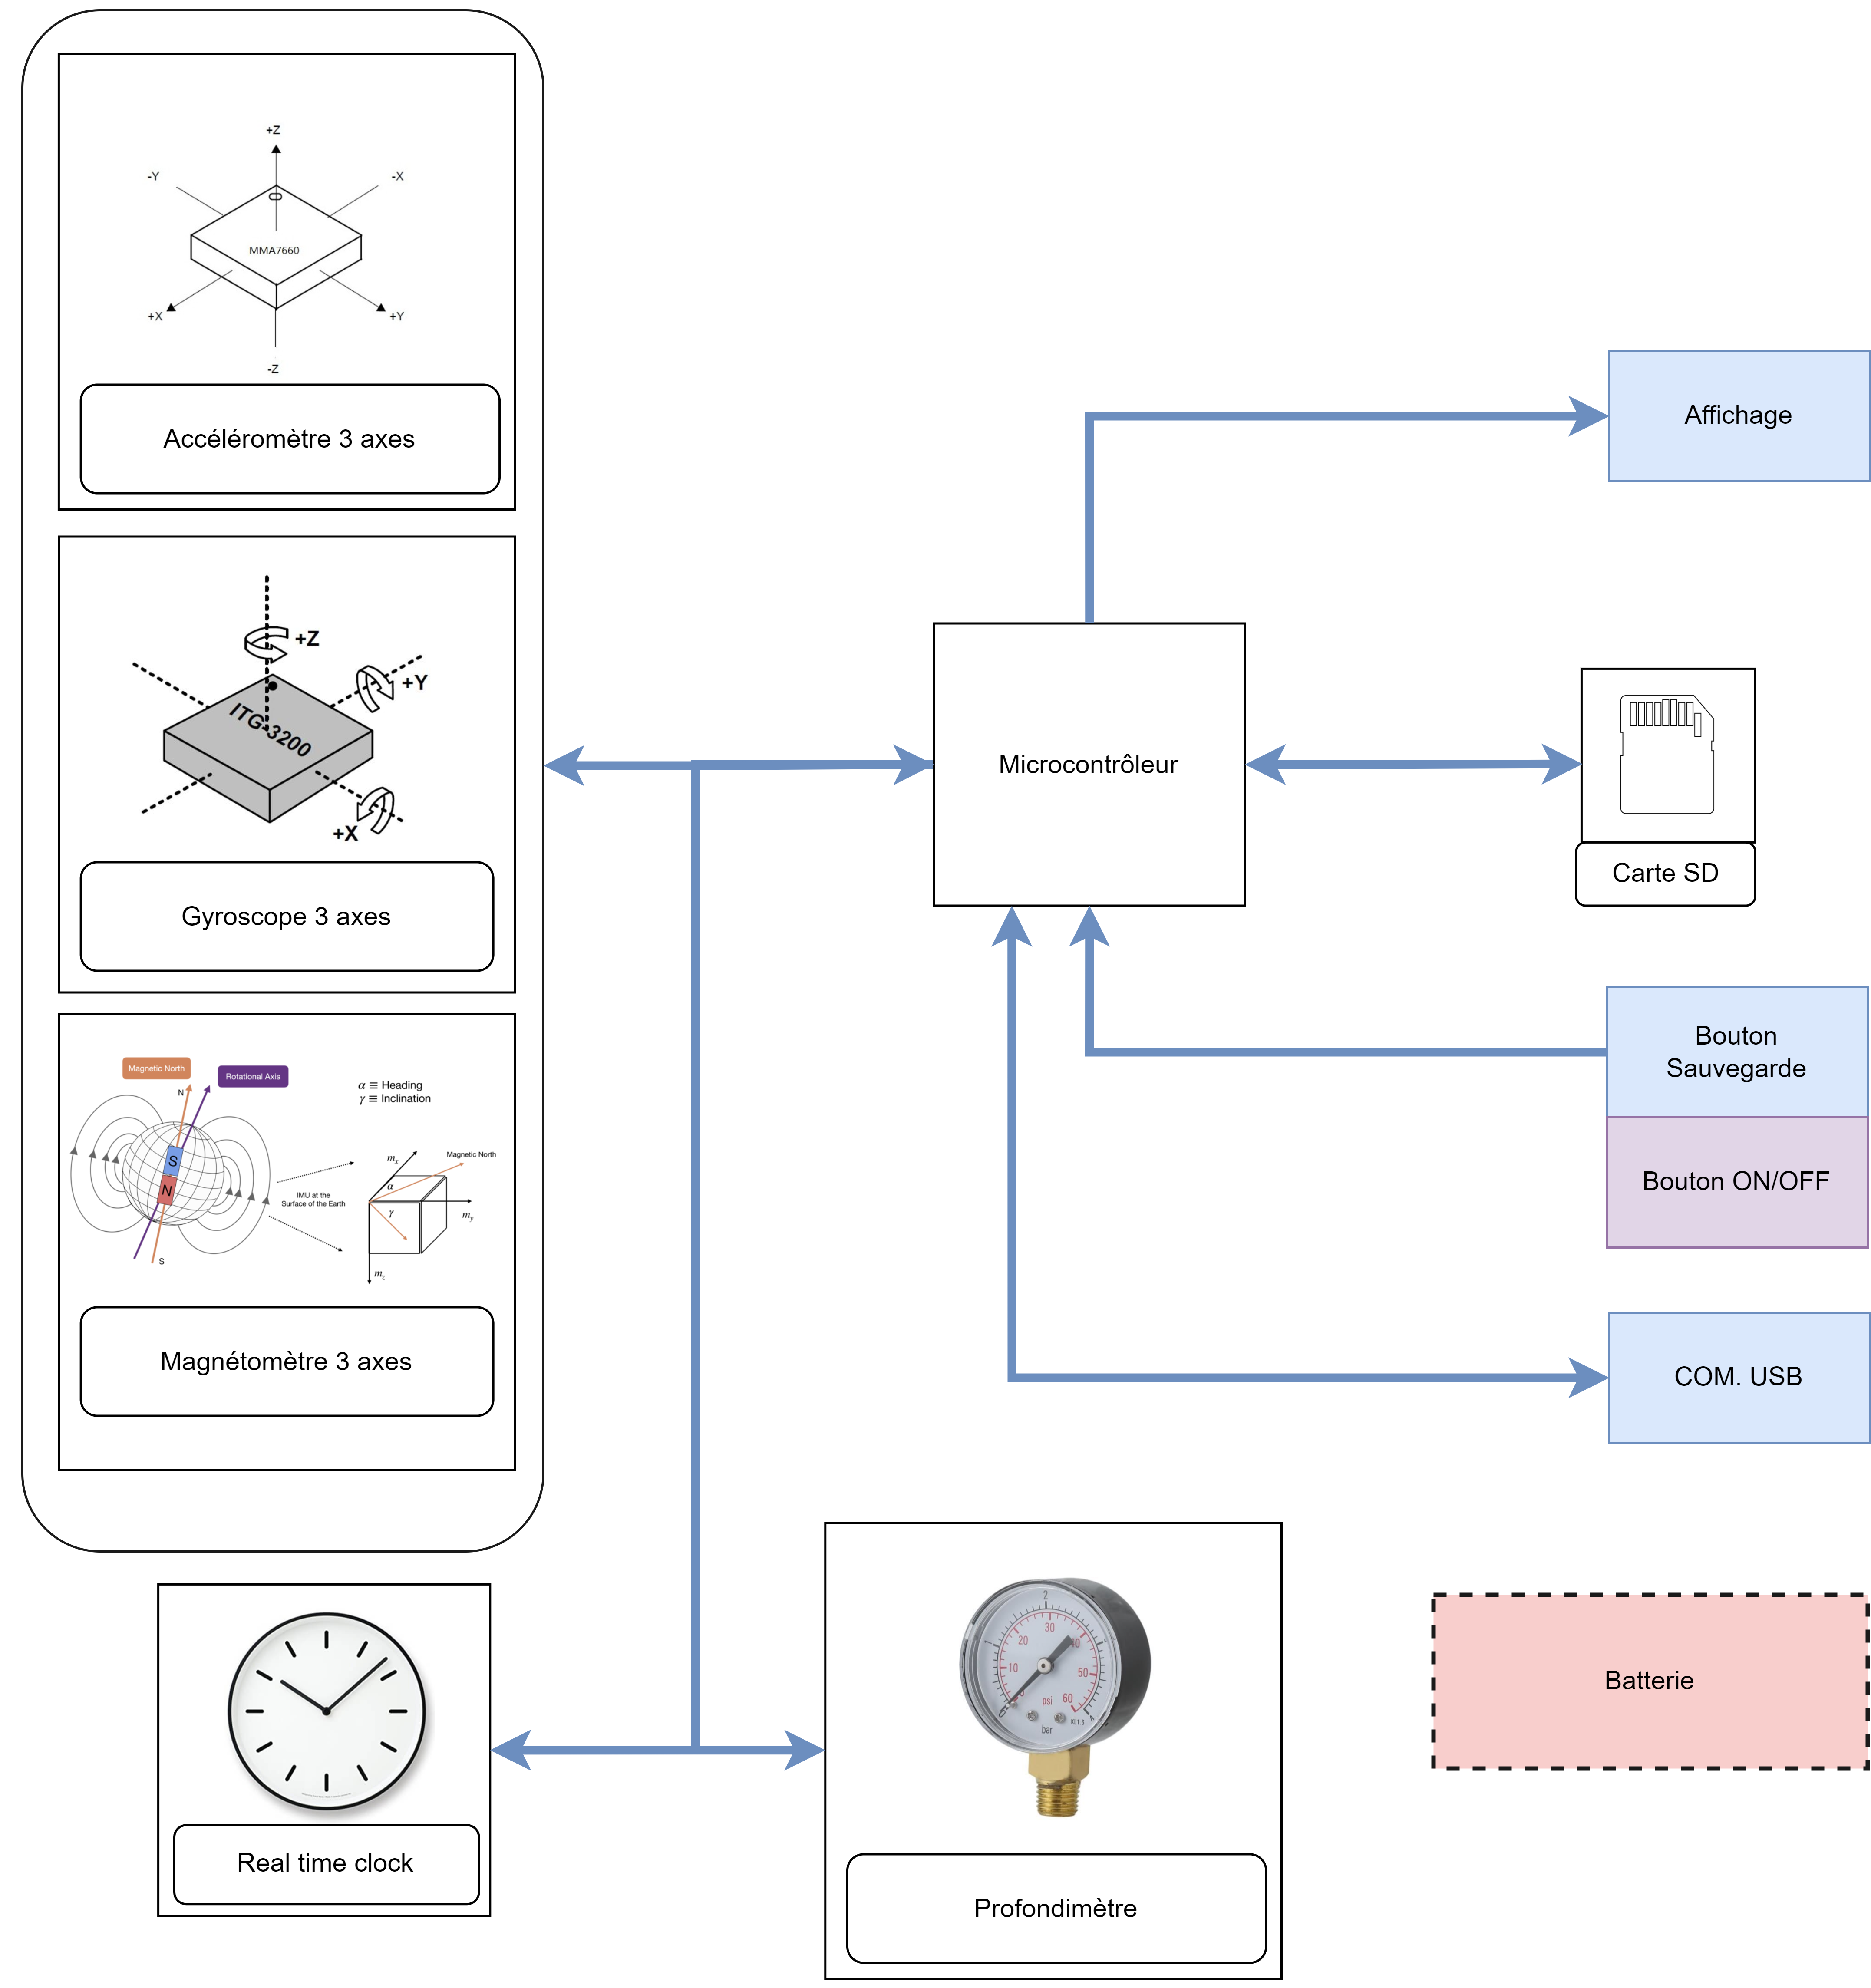
\includegraphics[width=.65\textwidth, center,]{../CDC/Figures/pre-etude.drawio.png}
    \caption{Schéma de principe}
    \source{Auteur}
\end{figure}
\clearpage

% ---- Description des blocs ----
\subsection{Description des blocs}
\begin{enumerate}
    \item \textbf{Carte SD :}\\
    Stockage des données de mesures chaque 100ms, cœur du projet.
    \item \textbf{Accéléromètre-gyroscope-magnétomètre :}\\
    Lecture des données individuelles brute ainsi que de fusion des capteurs, pour mesurer les déplacements sur 9 degrés de libertés.
    \item \textbf{Profondimètre :}\\
    Mesure la pression pour déduire la profondeur, afin de corroborer les autres mesures des capteurs.
    \item \textbf{Real time clock :}\\
    Permet de sauvegarder la temporalité du set de mesure dans la carte SD.
    \item \textbf{Affichage :}\\
    Affichage LED ou écran, pour affichage pas encore définis (ex. Profondeur, état batterie…)
    \item \textbf{Bouton sauvegarde :}\\
    Permet la mise en valeur d’un set de mesure. La forme de ce bouton n’est pas encore définie. Il sera peut-être fusionné avec le bouton ON/OFF.
    \item \textbf{Bouton ON/OFF :}\\
    Permet d’allumer ou d’éteindre le système.
    \item \textbf{Batterie :}\\
    Batterie du système, technologie à définir dans la pré-étude. 
    \item \textbf{COM. USB :}\\
    Permet de charger les batteries. Il faudra également prévoir dans cette version l’interface électronique pour la lecture de la carte SD directement par le port USB.
    \item \textbf{Microcontrôleur :}\\
    Lis et traite les valeurs des capteurs, sauvegarde dans la carte SD...
\end{enumerate}


\clearpage

% ---- JALONS ----
\subsection{Jalons principaux}
\begin{figure}[h!]
    \centering
    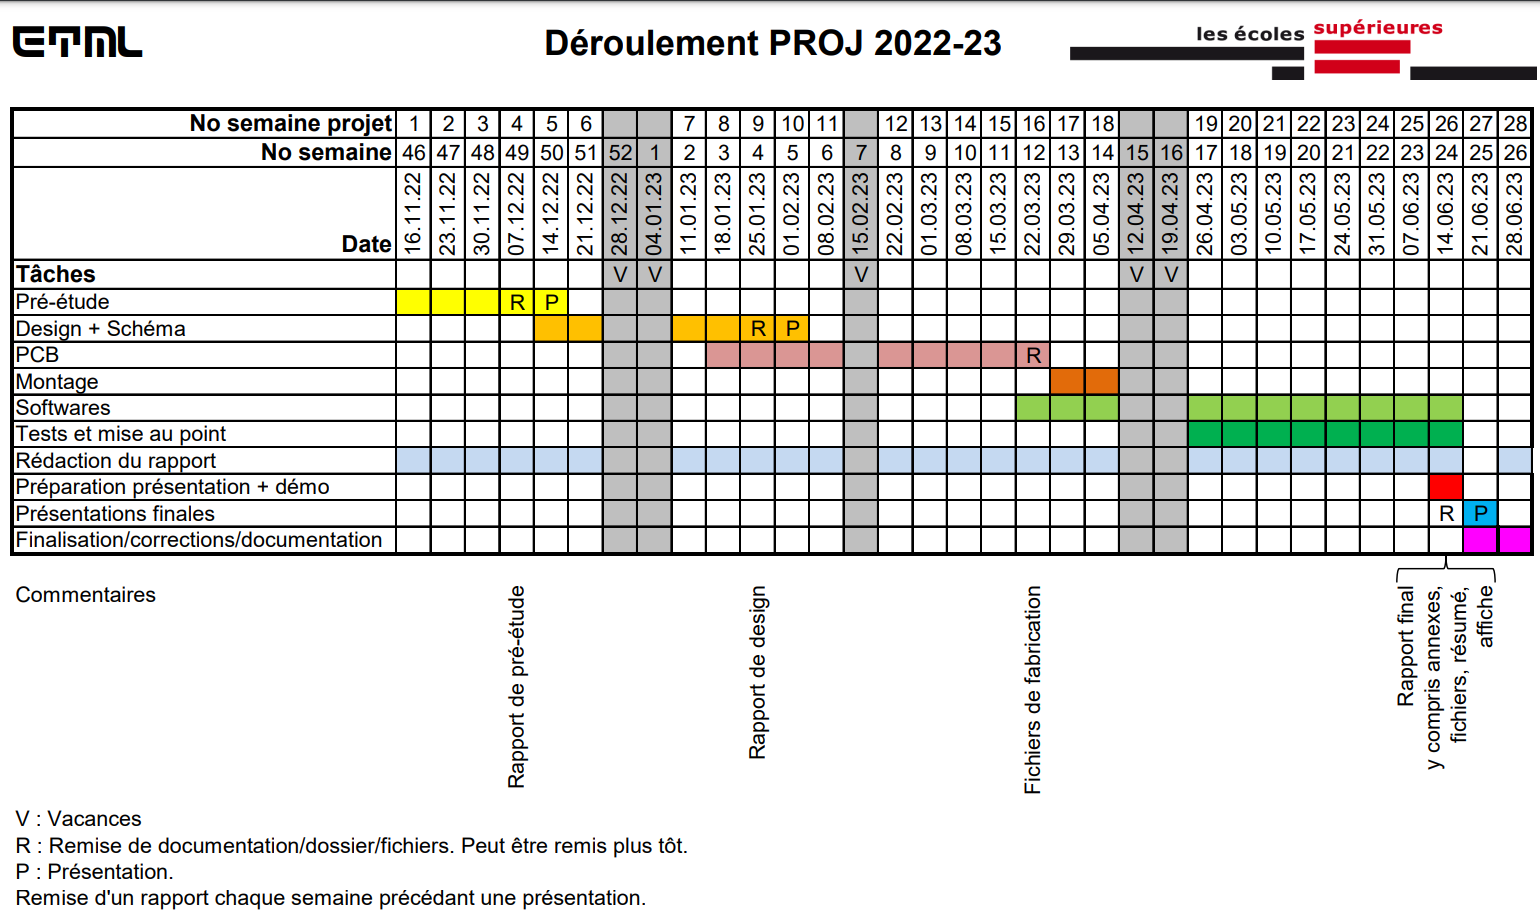
\includegraphics[width=.9\textwidth,center,]{../CDC/Figures/Tab-Jalons-PROJ.PNG}
    \caption{Jalons principaux}
    \label{fig:Jalons}
\end{figure}

\subsection{Livrable}
\begin{itemize}
    \item[•] Les fichiers sources de CAO électronique des PCB réalisés
    \item[•] Tout le nécessaire à fabriquer un exemplaire hardware de chaque :
    \item[•] fichiers de fabrication (GERBER) / liste de pièces avec références pour commande / implantation
    \item[•] Prototype fonctionnel
    \item[•] Modifications / dessins mécaniques, etc
    \item[•] Les fichiers sources de programmation microcontrôleur (.c  / .h)
    \item[•] Tout le nécessaire pour programmer les microcontrôleurs (logiciel ou fichier .hex)
    \item[•] Un calcul / estimation des coûts
    \item[•] Un rapport contenant les calculs - dimensionnement de composants - structogramme, etc.
\end{itemize}

\clearpage
